\documentclass[tikz,border=10pt]{standalone}
\usepackage{tikz}
\usetikzlibrary{shapes,arrows,positioning,fit,calc}

\begin{document}
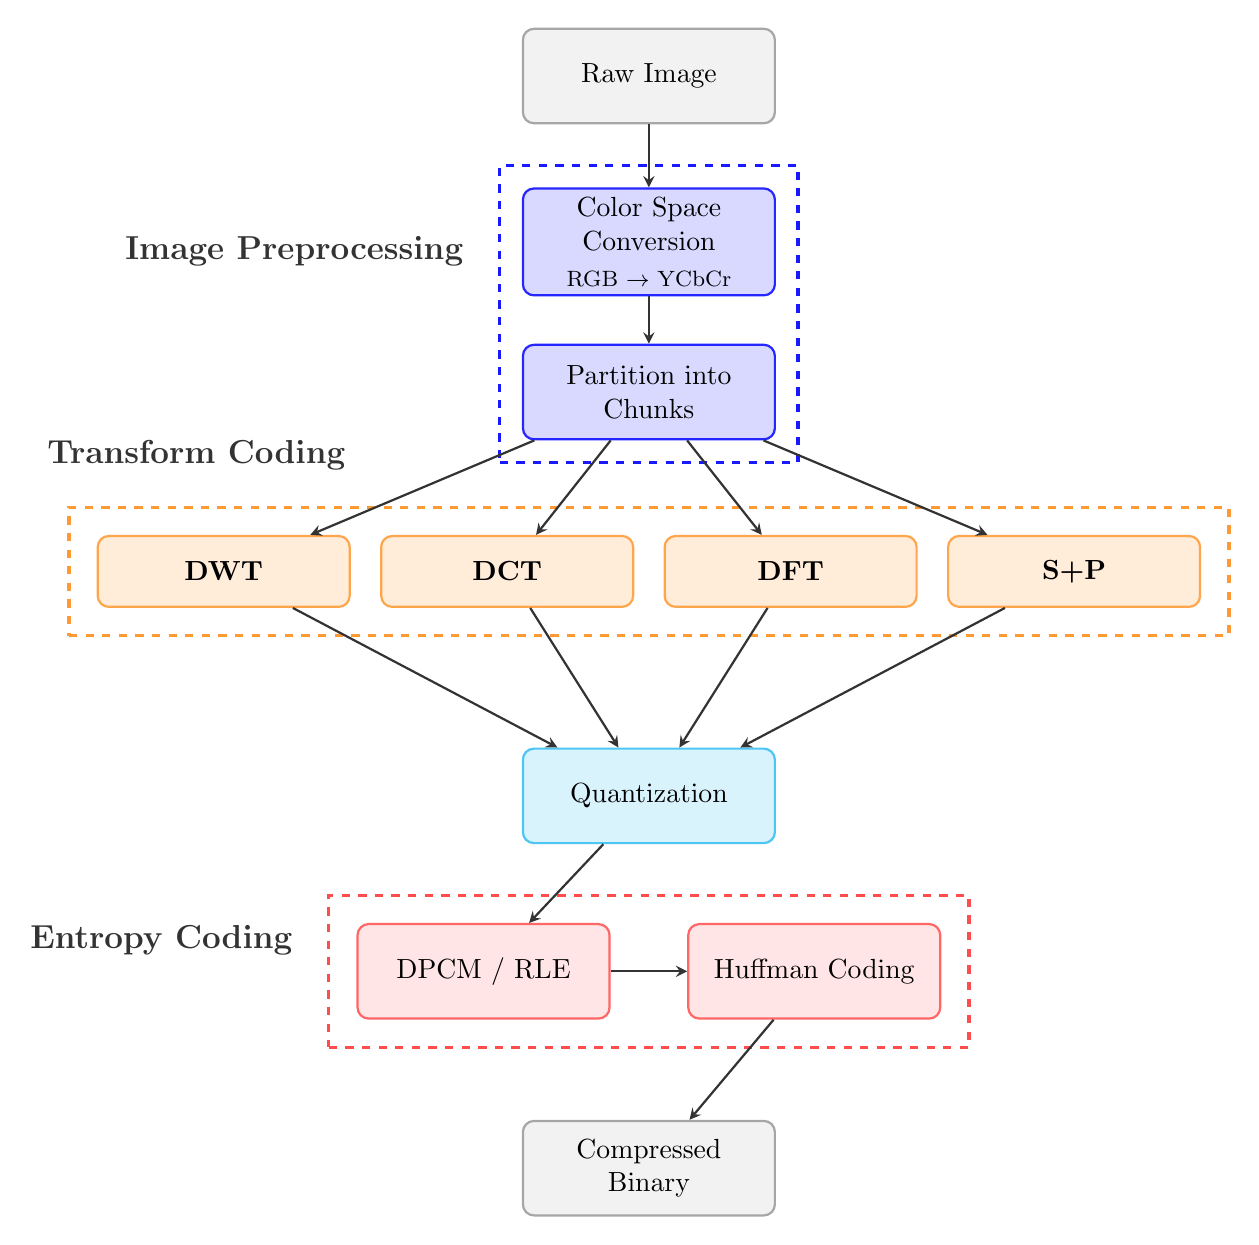
\begin{tikzpicture}[
  input/.style={rectangle,rounded corners=4pt,draw=gray!70,fill=gray!10,thick,
                minimum width=3.2cm,minimum height=1.2cm,align=center},
  process/.style={rectangle,rounded corners=4pt,draw=blue!85,fill=blue!15,thick,
                  minimum width=3.2cm,minimum height=1.2cm,align=center},
  transform/.style={rectangle,rounded corners=4pt,draw=orange!70,fill=orange!15,thick,
                    minimum width=3.2cm,minimum height=0.9cm,align=center,font=\bfseries},
  quant/.style={rectangle,rounded corners=4pt,draw=cyan!70,fill=cyan!15,thick,
                minimum width=3.2cm,minimum height=1.2cm,align=center},
  entropy/.style={rectangle,rounded corners=4pt,draw=red!60,fill=red!10,thick,
                  minimum width=3.2cm,minimum height=1.2cm,align=center},
  output/.style={rectangle,rounded corners=4pt,draw=gray!70,fill=gray!10,thick,
                 minimum width=3.2cm,minimum height=1.2cm,align=center},
  arrow/.style={->,>=stealth,thick,black!80},
  sectionlabel/.style={font=\small\bfseries,black!80,fill=white,inner sep=1pt}
]

% ===== INPUT =====
\node[input] (input) {Raw Image};

% ===== PREPROCESSING =====
\node[process,below=8mm of input] (colorspace) {Color Space\\Conversion\\[1pt]\footnotesize RGB $\rightarrow$ YCbCr};
\node[process,below=6mm of colorspace] (chunk) {Partition into\\Chunks};

\node[draw=blue!90,dashed,very thick,fit=(colorspace)(chunk),inner sep=8pt] (pre_box) {};
% title to the LEFT of the dashed box
\node[sectionlabel,anchor=east, font=\large\bfseries] at ($(pre_box.west)+(-4mm,8mm)$) {Image Preprocessing};

\draw[arrow] (input) -- (colorspace);
\draw[arrow] (colorspace) -- (chunk);

% ===== TRANSFORM CODING (parallel) =====
\node[transform,below=12mm of chunk,xshift=-5.4cm] (dwt) {DWT};
\node[transform,below=12mm of chunk,xshift=-1.8cm] (dct) {DCT};
\node[transform,below=12mm of chunk,xshift=+1.8cm]  (dft) {DFT};
\node[transform,below=12mm of chunk,xshift=+5.4cm] (sp) {S+P};

\node[draw=orange!80,dashed,very thick,fit=(dwt)(dct)(dft)(sp),inner sep=10pt] (tf_box) {};
% title to the LEFT of the dashed box
\node[sectionlabel,anchor=east, font=\large\bfseries] at ($(chunk.west)+(-22mm,-8mm)$) {Transform Coding};

\foreach \t in {dwt,dct,dft,sp} {
  \draw[arrow] (chunk) -- (\t);
}

% ===== QUANTIZATION =====
\node[quant,below=14mm of tf_box] (quant) {Quantization};
\foreach \t in {dwt,dct,dft,sp} {
  \draw[arrow] (\t) -- (quant);
}

% ===== ENTROPY CODING =====
\node[entropy,below=10mm of quant,xshift=-2.1cm] (dpcm) {DPCM / RLE};
\node[entropy,below=10mm of quant,xshift=+2.1cm] (huff) {Huffman Coding};

\node[draw=red!70,dashed,very thick,fit=(dpcm)(huff),inner sep=10pt] (ent_box) {};
% title to the LEFT of the dashed box
\node[sectionlabel,anchor=east, font=\large\bfseries] at ($(ent_box.west)+(-4mm,4mm)$) {Entropy Coding};

% correct arrows through entropy path
\draw[arrow] (quant) -- (dpcm);
\draw[arrow] (dpcm) -- (huff);

% ===== OUTPUT =====
\node[output,below=35mm of quant] (out) {Compressed\\Binary};
\draw[arrow] (huff) -- (out);

% (optional) figure title
% \node[font=\Large\bfseries] at ($(input)+(0,12mm)$) {Image Compression Pipeline};
% We dont need the title for the paper since figures are all already indexed and named

\end{tikzpicture}
\end{document}
